% !TEX root = ../gw.tex

%\suv{Hopefully after my comments are gone, the figures show up in correct sequence!}
\section{Experiments}\label{sec:experiments}

Algorithm~\ref{alg:gw} provides an extremely simple technique for optimizing the \GWa objective function.  We view this simplicity as an advantage; our algorithm is implementable in nearly any framework and generalizable to many classes of domains.  In this section, we verify that simplicity does not come at the cost of performance through experiments designed to reveal properties of our iterative technique.

\paragraph*{Convergence.}

\begin{figure}[t]\centering\pgfplotsset{scaled y ticks=false}
\begin{tikzpicture}
\begin{axis}[xlabel={\footnotesize Iteration},ylabel={\footnotesize \GWa objective},width=\columnwidth,height=.6\columnwidth,xlabel near ticks,ylabel near ticks,line cap = round,
line join = round,
xlabel shift = -.08in,
ylabel shift = -.08in,
xmin = 1,
xmax = 50,
yticklabel style={
        /pgf/number format/fixed,
        /pgf/number format/precision=3
},
scaled y ticks=false,legend cell align=left]
\addplot[mark=none,color=lightgray,thick,dotted] table[x index=0,y index=6,col sep=comma,mark=none,color=lightgray] {figures/eta/data_0.008.txt};\addlegendentry{\footnotesize $\eta=2$};
\addplot[mark=none,color=cyan,thick] table[x index=0,y index=5,col sep=comma,mark=none] {figures/eta/data_0.008.txt};\addlegendentry{\footnotesize $\eta=1$};
\addplot[mark=none,color=purple,thick] table[x index=0,y index=4,col sep=comma,mark=none] {figures/eta/data_0.008.txt};\addlegendentry{\footnotesize $\eta=2^{-1}$};
\addplot[mark=none,color=blue,thick] table[x index=0,y index=3,col sep=comma,mark=none] {figures/eta/data_0.008.txt};\addlegendentry{\footnotesize $\eta=2^{-2}$};
\addplot[mark=none,color=green,thick] table[x index=0,y index=2,col sep=comma,mark=none] {figures/eta/data_0.008.txt};\addlegendentry{\footnotesize $\eta=2^{-3}$};
\addplot[mark=none,color=red,thick] table[x index=0,y index=1,col sep=comma,mark=none] {figures/eta/data_0.008.txt};\addlegendentry{\footnotesize $\eta=2^{-4}$};
\end{axis}
\end{tikzpicture}\\\vspace{-.05in}
(a) $\alpha=8\times10^{-3}$\\\vspace{.05in}
%
%
\begin{tikzpicture}
\begin{axis}[xlabel={\footnotesize Iteration},ylabel={\footnotesize \GWa objective},width=\columnwidth,height=.6\columnwidth,xlabel near ticks,ylabel near ticks,line cap = round,
line join = round,
xlabel shift = -.08in,
ylabel shift = -.08in,
xmin = 1,
xmax = 50,
yticklabel style={
        /pgf/number format/fixed,
        /pgf/number format/precision=3
},
scaled y ticks=false,legend cell align=left]
\addplot[mark=none,color=cyan,thick] table[x index=0,y index=5,col sep=comma,mark=none] {figures/eta/data_0.0007.txt};\addlegendentry{\footnotesize $\eta=1$};
\addplot[mark=none,color=purple,thick] table[x index=0,y index=4,col sep=comma,mark=none] {figures/eta/data_0.0007.txt};\addlegendentry{\footnotesize $\eta=2^{-1}$};
\addplot[mark=none,color=blue,thick] table[x index=0,y index=3,col sep=comma,mark=none] {figures/eta/data_0.0007.txt};\addlegendentry{\footnotesize $\eta=2^{-2}$};
\addplot[mark=none,color=green,thick] table[x index=0,y index=2,col sep=comma,mark=none] {figures/eta/data_0.0007.txt};\addlegendentry{\footnotesize $\eta=2^{-3}$};
\addplot[mark=none,color=red,thick] table[x index=0,y index=1,col sep=comma,mark=none] {figures/eta/data_0.0007.txt};\addlegendentry{\footnotesize $\eta=2^{-4}$};
\end{axis}
\end{tikzpicture}\\\vspace{-.05in}
(b) $\alpha=7\times10^{-4}$
\vspace{-.1in}
\caption{Convergence for the examples in Figure~\ref{fig:reg}.\vspace{-.15in}}\label{fig:convergence}
\end{figure}

%\gabriel{Maybe I am misinterpreting the following paragraphe, but it seems to indicate that large $\eta$ helps to avoid local minimum, but the curve seems to indicate otherwise (small $\eta$ leads to better objective values). Can you explain ? }\justin{i removed a misleading "local" in the last sentence -- maybe this helps?}


Figure~\ref{fig:convergence} illustrates convergence of our algorithm on the experiments in Figure~\ref{fig:reg}, with several choices of $\eta$.  The experiments illustrate that the bound on $\eta$ in Proposition~\ref{prop:gw_convergence} is loose, that is, some choices of $\eta\geq\nicefrac{c\alpha}{1+c\alpha}$ still exhibit convergence.  In our experiments, the algorithm appears to converge monotonically even when $\eta=1$.  While we are unable to provide rigorous proof of convergence in this regime, from an engineering standpoint larger $\eta$ values can hasten completion time. Figure~\ref{fig:convergence}a shows an example with $\eta>1$ that does not converge.  As a trade-off, Figure~\ref{fig:convergence}b illustrates that the larger steps can skip past optima with better objective values; in this case, the different local optima correspond to different matchings of the octopus's tentacles.

\paragraph*{Sensitivity.}  

\begin{figure}[t]\centering\pgfplotsset{scaled y ticks=false}
%
%
\begin{tabular}{c@{}c@{}c}
\includegraphics[height=.2\linewidth]{figures/stability/source_bull.pdf}&
\includegraphics[height=.2\linewidth]{figures/stability/minAlphaTarget_cropped.pdf}&
\includegraphics[height=.2\linewidth]{figures/stability/maxAlphaTarget_cropped.pdf}\\
\small Source & \small$\alpha=5\times 10^{-4}$ &\small $\alpha=10^{-2}$
\end{tabular}
%
%
\begin{tikzpicture}
\begin{axis}[xlabel={\footnotesize $\alpha$},ylabel={\footnotesize Objective term},width=\columnwidth,height=.5\columnwidth,
%xlabel near ticks,
ylabel near ticks,
line cap = round,
line join = round,
xlabel shift = -.08in,
ylabel shift = -.08in,
xmin = 0.001,
xmax = .1,
ymin = .2,
yticklabel style={
        /pgf/number format/fixed,
        /pgf/number format/precision=3
},xmode=log,%ymode=log,
scaled y ticks=false,legend cell align=left,legend pos = north west]
\addplot[only marks,color=blue,mark size = .3] table[x index=0,y index=1,col sep=comma,mark=none] {figures/stability/initialGuess.txt};\addlegendentry{\footnotesize $\langle \G,\bL(\G)\rangle$};
\end{axis}
\end{tikzpicture}\\\vspace{-.075in}
(a) Triangle mesh matching ($n_0=n=502$)\\
\vspace{.1in}\hrule
\vspace{.1in}
%
%
\begin{tabular}{cccc}
\includegraphics[height=.2\linewidth]{figures/stability/source2d.pdf}&
\includegraphics[height=.2\linewidth]{figures/stability/target2d1.pdf}&
\includegraphics[height=.2\linewidth]{figures/stability/target2d2.pdf}&
\includegraphics[height=.2\linewidth]{figures/stability/target2d3.pdf}\\
\small Source & \small$\alpha=5\times 10^{-4}$ &\small $\alpha=5\times 10^{-4}$&\small$\alpha=2\times10^{-2}$\vspace{-.05in}\\
& \small\emph{(trial 1)} & \small\emph{(trial 2)}
\end{tabular}\vspace{-.05in}
%
%
\begin{tikzpicture}
\begin{axis}[xlabel={\footnotesize $\alpha$},ylabel={\footnotesize Objective term},width=\columnwidth,height=.5\columnwidth,
%xlabel near ticks,
ylabel near ticks,
line cap = round,
line join = round,
xlabel shift = -.08in,
ylabel shift = -.08in,
xmax = 0.001,
xmin = .0006,
ymin = 0.002,
ymax = .004,
yticklabel style={
        /pgf/number format/fixed,
        /pgf/number format/precision=3
},xmode=log,%ymode=log,
scaled y ticks=false,legend cell align=left,legend pos = north west]
\addplot[only marks,color=blue,mark size = .3] table[x index=0,y index=1,col sep=comma,mark=none] {figures/stability/initialGuess2.txt};\addlegendentry{\footnotesize $\langle \G,\bL(\G)\rangle$};
\end{axis}
\end{tikzpicture}\\\vspace{-.075in}
(b) 2D point sample matching ($n_0=119$, $n=121$)
%
%
\caption{Sensitivity to initial guess of $\G$ for matching (a) surfaces and (b) planar point samples.\vspace{-.2in}}\label{fig:sensitivity}
\end{figure}

Since Algorithm~\ref{alg:gw} optimizes a non-convex objective, the output may depend on the initial $\G$. Figure~\ref{fig:sensitivity} tests sensitivity to the initial guess.  Like the previous test, for a given matching task we plot the optimized GW objective $\langle \G,\bL(\G)\rangle$ as a function of $\alpha$; this roughly should increase as $\alpha$ increases.  In this test, however, we randomly generate an initial $\G$ in each trial.% rather than using the matrix of all ones suggested in Algorithm~\ref{alg:gw}.

We evaluate surface matching stability in Figure~\ref{fig:sensitivity}a; distance matrices $\D_0,\D$ contain geodesic distances.  This test, representative of many similar experiments involving surfaces, shows little dependence on the initial $\G$ even for sharp matchings (low $\alpha$), as reflected by the single coherent curve of objective values.

To reveal a case where multiple optima appear, we consider the task of matching two Poisson disk samples from a right triangle in Figure~\ref{fig:sensitivity}b; here, $\D_0,\D$ contain planar Euclidean distances.  Since the triangle has a reflectional symmetry, we expect there to be two nearly-optimal maps from the source to the target.  When $\alpha$ is sufficiently small, we do observe two different optimized objectives for the same $\alpha$ depending on which symmetric map is closer to the initial estimate of $\G$.  For large enough $\alpha$ (displayed above the plot), the optimal coupling superposes the two optimal maps and the two parallel curves merge.

\paragraph*{Efficiency.}  

\begin{figure}[t]\centering
\begin{tikzpicture}
\begin{axis}[xlabel={\footnotesize Time (sec.)},ylabel={\footnotesize \GWa objective},width=\columnwidth,height=.6\columnwidth,
ylabel near ticks,xlabel near ticks,
line cap = round,
line join = round,
xlabel shift = -.08in,
ylabel shift = -.08in,
xmin = 0,
xmax=5,
ymin = 0,
ymax = .05,
yticklabel style={
        /pgf/number format/fixed,
        /pgf/number format/precision=3
},
legend style = {row sep =-.05in, inner sep = .01in,anchor=south east,at={(.98,.15)}},
scaled y ticks=false,legend cell align=left,
%legend pos = south east
]
\addplot[color=red,mark size = 1,dashed,mark=*] table[x index=0,y index=1,col sep=comma] {figures/efficiency/bfgs119alpha0.001.txt};\addlegendentry{\footnotesize BFGS, $n_0\!=\!n\!=\!119$};
\addplot[color=red,mark size = 1,mark=*] table[x index=0,y index=1,col sep=comma] {figures/efficiency/gw119alpha0.001.txt};\addlegendentry{\footnotesize GW, $n_0\!=\!n\!=\!119$};
\addplot[color=blue,mark size = 1,mark=*,dashed] table[x index=0,y index=1,col sep=comma] {figures/efficiency/bfgs333alpha0.001.txt};\addlegendentry{\footnotesize BFGS, $n_0\!=\!n\!=\!333$};
\addplot[color=blue,mark size = 1,mark=*] table[x index=0,y index=1,col sep=comma] {figures/efficiency/gw333alpha0.001.txt};\addlegendentry{\footnotesize GW, $n_0\!=\!n\!=\!333$};
\end{axis}
\end{tikzpicture}\\\vspace{-.15in}
\caption{Objective value vs.\ time for triangular samples as in Figure~\ref{fig:sensitivity}b ($\alpha\equiv10^{-3}$); markers indicate iterations.}\label{fig:efficiency}
\end{figure}

Figure~\ref{fig:efficiency} tests efficiency of our technique.  Here, we plot the \GWa objective as a function of time, measured using a single-threaded implementation in Matlab on a 2.1 GHz Intel i7 CPU with 8GB memory.  \cite{memoli-2011} and subsequent works mention two optimization algorithms (without regularization):  gradient descent and alternation.  The latter solves an optimal transportation-style linear program in each step.  Our method directly improves that technique, so to compare to a more distant alternative we consider gradient-based routines popular in graphics.  In particular, we employ a standard implementation of the interior point method~\cite{waltz-2006} with ``limited-memory'' BFGS Hessian estimates.  Both in terms of elapsed time and number of iterations, our method reaches a critical point far faster than the interior point alternative.  The difference widens as the size of the problem increases.
%\suv{What would be a competing fast method that the reviewers may know about?}%for GW?  Just BFGS I think...Graphics is a relatively late arriver to the optimization world.

\paragraph*{Robustness.} To demonstrate the robustness of $\GWa$-based matching, Figure~\ref{fig:more_maps} illustrates couplings between pairs of triangulated surfaces computed using our algorithm.  Even when the surfaces undergo significant geometric and topological changes (e.g.\ adding slats to the chair backs and matching a cup to a mug twice its height) that deviate considerably from isometry, conformality, and other assumptions imposed by surface matching algorithms, our method stably recovers a reasonable correspondence.  We visualize  maps by showing rows of the measure coupling color coded on a target from corresponding points on a source. %using the method proposed in~\cite[Fig.\ 10]{solomon-2015}, but in contrast to their method for correspondence our algorithm (1) does not need ground truth correspondences or feature descriptors and (2) runs in a small fraction of their reported runtimes.

% \suv{Should this type of capability not be highlighted earlier on in contributions?}% Comparing against my old paper is probably not much of a contribution --- not sure anyone uses it :-) --- but added myself a to-do to mention in the contributions

\begin{figure*}\centering
\setlength{\fboxsep}{0pt}%
\setlength{\fboxrule}{1pt}%
\fbox{
\!\includegraphics[height=.11\linewidth]{figures/surface_maps/source_hands.pdf}
\!\includegraphics[height=.11\linewidth]{figures/surface_maps/target_hands.pdf}
\!}
\fbox{
\!\includegraphics[height=.15\linewidth]{figures/surface_maps/source_chair.pdf}
\!\includegraphics[height=.15\linewidth]{figures/surface_maps/target_chair.pdf}
\!}
\fbox{
\!\includegraphics[height=.15\linewidth]{figures/surface_maps/source_human.pdf}
\!\includegraphics[height=.15\linewidth]{figures/surface_maps/target_human.pdf}
\!}
\fbox{
\!\includegraphics[height=.15\linewidth]{figures/surface_maps/source_humantostick.pdf}
\!\includegraphics[height=.15\linewidth]{figures/surface_maps/target_humantostick.pdf}
\!}
\fbox{
\!\includegraphics[height=.11\linewidth]{figures/surface_maps/source_mugs.pdf}
\!\includegraphics[height=.11\linewidth]{figures/surface_maps/target_mugs.pdf}
\!}
\caption{Additional surface correspondences computed using Algorithm~\protect\ref{alg:gw} ($\alpha\!\equiv\!5\!\times\!10^{-4},\eta\!\equiv\!1$).  As in~\protect\cite{solomon-2015},  colored points on the left are mapped to colored distributions on the right.  \S\ref{sec:symmetry} details a method for addressing the symmetry reversal in the third map.\vspace{-.15in}}\label{fig:more_maps}
\end{figure*}

\paragraph*{Generality.} Throughout this paper, we attempt to demonstrate our algorithm on a variety of matching tasks.  In this section, we highlight a few additional examples to underscore its wide applicability.

%\begin{figure}[t]\centering % became the teaser
%\begin{tabular}{c@{\hspace{.25in}}c}
%\includegraphics[height=.5\linewidth]{figures/icon/icon_source.pdf}&
%\includegraphics[height=.5\linewidth]{figures/icon/icon_target.pdf}
%\end{tabular}
%\caption{Mapping a 3D model onto a 2D icon ($n_0\!=\!2002,n\!=\!2315,\alpha\!=\!3\times10^{-5}$).}\label{fig:shape_to_icon}
%\end{figure}
Figure~\ref{fig:shape_to_icon} (page 1) tests our algorithm's flexibility to domain class.  Here, we map a triangle mesh to five different classes of target domains.  Despite the contrasting structures and even dimensionalities of the targets, our algorithm extracts a meaningful correspondence.

\begin{figure}[t]\centering
\begin{tabular}{c@{\hspace{.25in}}c}
\includegraphics[height=.5\linewidth]{figures/graph_to_shape/graph.pdf}&
\includegraphics[height=.5\linewidth]{figures/graph_to_shape/alligator_target.pdf}
\end{tabular}
\caption{Mapping a graph onto a shape ($n_0\!=\!27,n\!=\!2502,\alpha\!=\!1.8\times10^{-4}$).\vspace{-.15in}}\label{fig:graph_to_shape}
\end{figure}
Similarly, Figure~\ref{fig:graph_to_shape} shows an example of mapping a graph onto a surface.  Here, distances $\D_0$ on the graph are all-pairs shortest-path distances with unit edge weights, and $\D$ contains geodesic distances on the target surface.  Convergence for this example was particularly fast given the small size of the source domain.

\begin{figure}[t]\centering
\includegraphics[height=\linewidth]{figures/image_grid/imageLayout.pdf}
\caption{Mapping 196 images onto a $14\times14$ image grid while preserving color similarity. \small{(Images from Flickr public domain collection.)}\vspace{-.15in}}\label{fig:images}
\end{figure}

Figure~\ref{fig:images} applies our machinery to mapping a set of images onto a grid layout; as a point of comparison, Fried et al.~\shortcite{fried-2015} recently proposed a more complicated optimization routine for the same problem.  Here, $\D_0$ contains distances between average \textsc{Lab} color over an image, and $\D$ contains Euclidean distances between grid cells.  For this application, we need to extract a matching rather than a soft measure coupling $\G$.  To do so, after optimizing for $\G$, we solve a linear assignment problem
$$
\begin{array}{rl}
\max_{\tilde\G} & \langle \tilde \G,\G\rangle\\
\textrm{s.t.} & \tilde\G\geq0\\
&\tilde\G\1=\1n\hspace{.25in}\tilde\G^\top\1=\1n_0.
\end{array}
$$
When $n_0=n$, this linear program admits a permutation matrix solution computable using a standard convex optimization tool or any of the many fast solvers for assignment problems.%\suv{Or using any of the 10s of fast solvers that exist for assignment problems.}

\setlength{\columnsep}{2pt}
\begin{wrapfigure}[9]{r}{0.23\textwidth}\centering
\vspace{-.15in}
\begin{tabular}{c@{}c}
\includegraphics[height=.6\linewidth]{figures/cloud/source_cloud.pdf}&
\includegraphics[height=.6\linewidth]{figures/cloud/cloud.pdf}
\end{tabular}
\vspace{-.15in}
\caption{Point clouds.}\label{fig:clouds}
\end{wrapfigure}
Figure~\ref{fig:clouds} shows an example matching a triangle mesh to a point cloud.  Here, we match a noisy and sparse point cloud face scan to a generic mesh of a face. Since the two shapes are in approximately the same pose, we take $\D_0, \D$ to contain Euclidean (rather than geodesic) distances.  We use mesh-based area weights on the source and uniform area weights on the target.  The match is successful despite the nonuniform sampling of the point cloud and a missing patch on the nose.

%\begin{figure}[t]\centering
%\fbox{\includegraphics[scale=.1]{figures/2d_shape_match/source.pdf}}\ \ \foreach \n in {1,...,4}{\includegraphics[scale=.09]{figures/2d_shape_match/target\n.pdf}\ \ }\\
%\fbox{\includegraphics[scale=.1]{figures/2d_shape_match/source_glass.pdf}}\ \ \foreach \n in {1,...,4}{\includegraphics[scale=.1]{figures/2d_shape_match/target_glass\n.pdf}\ \ }\\
%\fbox{\includegraphics[scale=.1]{figures/2d_shape_match/source_heart.pdf}}\ \ \foreach \n in {1,...,4}{\includegraphics[scale=.12]{figures/2d_shape_match/target_heart\n.pdf}\ \ }\\
%\fbox{\includegraphics[scale=.1]{figures/2d_shape_match/source_fork.pdf}}\ \ \foreach \n in {1,...,4}{\includegraphics[scale=.1]{figures/2d_shape_match/target_fork\n.pdf}\ \ }
%\caption{2D shape matching; color on the boxed model is transferred to the remaining models ($\alpha\equiv7.5\times10^{-4}$); results on full dataset in supplemental material.}\label{fig:2d_shape}
%\end{figure}

\setlength{\columnsep}{2pt}
\begin{wrapfigure}[7]{r}{0.12\textwidth}\centering
\vspace{-.15in}
\begin{tabular}{cc}
\includegraphics[height=.9\linewidth]{figures/2d_shape_match/source_fuzzy_fork.pdf}&
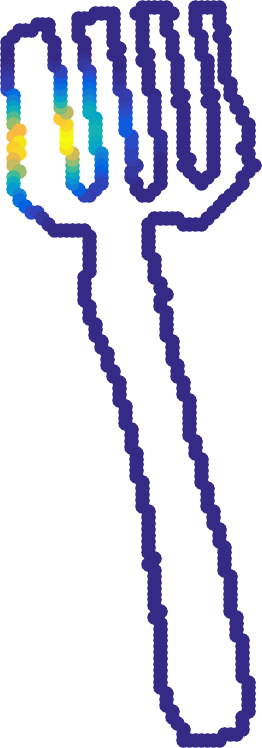
\includegraphics[height=.9\linewidth]{figures/2d_shape_match/target_fuzzy_fork.pdf}
\end{tabular}
\vspace{-.15in}
\caption{}\label{fig:forks}
\end{wrapfigure}
%Figure~\ref{fig:2d_shape} shows 
The supplemental document includes a 2D shape matching test (data from~\cite{thakoor-2007}).  The shapes are point clouds without topology.  We use the rounding procedure outlined for image layout to display the maps, transferring colors from the matched point on a source shape (boxed). Our algorithm recovers smooth maps for most 2D test cases.  The most challenging test in the dataset is the ``fork'' class; these shapes admit symmetries \emph{and} thin structures that make it difficult to extract a point-to-point map after applying the entropic regularizer.  Figure~\ref{fig:forks} shows an example before rounding.

%\paragraph*{Validation.} \justin{Hoping Vova can think of some dataset to test on.}

\paragraph*{Comparison.}  Here we provide a few examples qualitatively demonstrating how our method differs from existing work.

\begin{figure}[t]\centering\renewcommand{\arraystretch}{0.8}% Tighter
\begin{tabular}{@{}c@{\hspace{.1in}}c|c@{\hspace{.1in}}c@{}}
\includegraphics[height=.13\linewidth]{figures/sdp/sdp1.pdf}&
\includegraphics[height=.17\linewidth]{figures/sdp/sdp2.pdf}&
\includegraphics[height=.13\linewidth]{figures/sdp/gw1.pdf}&
\includegraphics[height=.17\linewidth]{figures/sdp/gw2.pdf}\\
Test 1 & Test 2 & Test 1 & Test 2\\
\tiny$\lambda_1\!=\!7,\lambda_2\!=\!0$
&
\tiny$\lambda_1\!=\!4,\lambda_2\!=\!3$
&
\tiny 6 iterations
&
\tiny 14 iterations
\\\hline
\multicolumn{2}{|c|}{\small \cite{kezurer-2015}, 2499 variables}&
\multicolumn{2}{c|}{\small $\GWa$, $\alpha\!=\!10^{-3}$, 49 variables}\\\hline
\end{tabular}
\caption{Comparison to SDP matching.  The points on the left of the vertical dotted lines are mapped to the right; edge darkness indicates value of $\G$.  The two largest eigenvalues are shown for~\protect\cite{kezurer-2015}; the second test case is not tight.  The number of iterations for six digits of precision is shown for \GWa.}\label{fig:sdp}
\end{figure}
Figure~\ref{fig:sdp} compares to~\cite{kezurer-2015} for a 2D matching problem using pairwise Euclidean distances.  We show a symmetric test case and an asymmetric test case.  For fair comparison, we use their SDP relaxation on the GW objective.  Our unoptimized implementation instantiated 2499 variables to match seven points using their method, which has $O(n^4)$ variables for $n$ matched points.  Beyond an obvious difference in timings, their relaxation was not tight in the symmetric test.  %; in their notation, the output  satisfied $Y\neq[X][X]^\top$.  
While optimization via the interior point method recovered a map that arbitrarily superposed the two equally optimal maps, the weights of the superposition were not isotropic or controllable.  Our method recovered a sharp map; the symmetric map can be recovered as described in \S\ref{sec:symmetry}.

The supplemental document includes a comparison to~\cite{aflalo-2015} in which we minimize $\|\D_0\G-\G\D\|_{\mathrm{Fro}}$ over doubly stochastic $\G$.  To match their setup, we assume $n_0\!=\!n$ with uniform area weights.  Although their method does not require an SDP, the convexity of their objective is problematic for (nearly-)symmetric domains; see the supplemental document for discussion.

\setlength{\columnsep}{1pt}
\begin{wrapfigure}[10]{r}{0.3\textwidth}\centering\centering\renewcommand{\arraystretch}{0.8}% Tighter
\vspace{-.15in}
\begin{tabular}{@{}c@{}c@{}c@{}}
\includegraphics[height=.25\linewidth]{figures/bim/bimSource.pdf}&
\includegraphics[height=.5\linewidth]{figures/bim/bimTarget.pdf}&
\includegraphics[height=.5\linewidth]{figures/bim/gwTarget.pdf}\\
\small Source & \small BIM & \small \GWa
\end{tabular}
\vspace{-.15in}
\caption{Blended intrinsic maps.}\label{fig:bim}
\end{wrapfigure}
Figure~\ref{fig:bim} compares to the Blended Intrinsic Maps (BIM) method of~\cite{kim-2011} for triangle mesh correspondence.  BIM constructs point-to-point maps between triangulated surfaces by patching together conformal (angle-preserving) maps.  For comparison, we compute a sharp \GWa map ($\alpha\!=\!5\!\times\!10^{-4}$) and show the highest-probability match for each source point.  Because BIM restricts to conformal maps rather than minimizing a measure of stretch like $\GWa$, it cannot capture the stretch of the neck and legs from the bull source model to the giraffe target.  \GWa more evenly distributes the distortion.

\begin{figure}[t]\centering
\begin{tikzpicture}
\begin{axis}[xlabel={\footnotesize Geodesic error},ylabel={\footnotesize \% correspondences},width=.8\columnwidth,height=.6\columnwidth,
ylabel near ticks,xlabel near ticks,
line cap = round,
line join = round,
xlabel shift = -.04in,
ylabel shift = -.08in,
xmin = 0,
xmax=.25,
ymin = 0,
ymax = 100,
yticklabel style={
        /pgf/number format/fixed,
        /pgf/number format/precision=3
},
xticklabel style={
        /pgf/number format/fixed,
        /pgf/number format/precision=3
},
legend style = {row sep =-.05in, inner sep = .01in,anchor=south east,at={(.98,.15)}},
scaled y ticks=false,legend cell align=left,
%legend pos = south east
]
\addplot[color=blue] table[x index=0,y index=1,col sep=comma] {figures/correspondence_benchmark/scape.txt};\addlegendentry{\footnotesize SCAPE};
\addplot[color=red] table[x index=0,y index=1,col sep=comma] {figures/correspondence_benchmark/shrec.txt};\addlegendentry{\footnotesize SHREC '07 animals};
\end{axis}
\end{tikzpicture}\\\vspace{-.2in}
\caption{Benchmark tests from~\protect\cite{kim-2011}.\vspace{-.2in}}\label{fig:benchmarks}
\end{figure}

Figure~\ref{fig:benchmarks} illustrates performance on benchmarks from~\cite{kim-2011}; the units of the plots and experiments are identical to the ones used in their paper to ease comparison to~\cite{kim-2011} and follow-on work.  For these experiments, we round measure couplings to sharp maps by mapping source points to the maximum of their corresponding rows in the coupling.  Despite our method's generality and design for rough rather than dense correspondence, it behaves comparably to algorithms for dense, isometry-invariant mapping on the near-isometric SCAPE dataset.  Error is higher the non-isometric SHREC '07 dataset; for some geometrically diverse surface pairs, \GWa takes the front of one animal to the back of another.  While the plots show results without user guidance, these negative results could easily be addressed using the supervised matching pipeline outlined in \S\ref{sec:supervised_matching}.  